\documentclass[%
	%draft
	]{ijsra}
\def\IJSRAidentifier{\currfilebase} %<---- don’t change this!
%-------Title | Email | Keywords | Abstract-------------
\def\shorttitle{Australian Archaeological Association 2016}
\def\maintitle{Australian Archaeological Association 2016\\ Conference Review}
\def\cmail{rhaw9263@uni.sydney.edu.au}
\def\keywords{Conference review, Australian Archaeology, Australian Archaeological Association, student input}
%\def\keywordname{}%<--- redefine the name “Keywords“ in needed language
\def\abstract{The Australian Archaeological Association (AAA) conference is an annual conference aiming to encourage the advancement of archaeology in Australia. The 39th AAA conference was held in the coastal town of Terrigal, New South Wales and for the first time in its history it was hosted by an Indigenous organisation; the Darkinjung Local Aboriginal Land Council (LALC). This defining moment in the history of AAA conferences and along with the theme “Interwoven: Indigenous and Western Knowledge in Archaeology and Heritage” promoted collaboration and understanding of different ways to explore Australian archaeology.}
%--------Author’s names------------
\def\authorone{Rebekah Hawkins}
\def\authortwo{Jacqueline Matthews}%<---- comment or delete if you do not need a second author.
\def\authorthree{Francesca McMaster}%<---- comment or delete if you do not need a third author.
%\def\authorfour{}%<---- comment or delete if you do not need a fourth author.
%\def\authorfive{}%<---- comment or delete if you do not need a fifth author.
%-------Biographical information-------------
\def\bioone{Rebekah Hawkins is currently undertaking honours in archaeology at the University of Sydney after recently graduating with a combined Bachelor of Arts (Archaeology) and Bachelor of Science (Anatomy and Geology). Her honours project is a lithic assemblage from Lake George in NSW, Australia with a focus on raw material quality and its influence on the size and shape of artefacts as well as changes in raw material quality throughout time. She is a Student Representative for the Australian Archaeological Association, on the Advisory board for the National Archaeology Student Conference after having chaired the conference in 2015 and is on the committee for National Archaeology Week Australia. While completing honours she is also working for archaeological consultancies in Sydney, Australia.}
\def\biotwo{Jacqueline recently graduated with a Master of Philosophy from the University of Western Australia where her research explored the intersections of relational ontology, social learning, and Australian Aboriginal lithic technology. She also holds a Bachelor of Arts with Honours from the University of Queensland. Her research interests include postcolonial, Indigenous and theoretical archaeologies focused on practical and collaborative applications in the Australian context. She was made a Life Member of the Australian Archaeological Association in 2016 and is an Associate Member of the Australian Association of Consulting Archaeologists having worked in cultural heritage management for five years.}%<---- comment or delete if there is no second author.
\def\biothree{Francesca McMaster recently graduated from the University of Sydney with first class honours in archaeology and a Bachelor of Arts in archaeology and art history. Her thesis research focused on the application of ethnography in Indigenous Australian archaeological interpretation. Her general research interests include the role of archaeology in the formation of concepts of nationalism and identity, including but not limited to, the use of analogy within archaeological interpretation and the continuing influence of colonisation in archaeology. Francesca currently works for museums and archaeological consultancies in Sydney, Australia.}%<---- comment or delete if there is no third author.
%\def\biofour{}%<---- comment or delete if there is no fourth author.
%\def\biofive{}%<---- comment or delete if there is no fifth author.
%------University/Institution--------------
\def\affilone{University of Sydney}
\def\affiltwo{University of Western Australia}%<---- comment or delete if there is no second author.
%\def\affilthree{University of Sydney}%<---- comment or delete if there is no third author.
%\def\affilfour{}%<---- comment or delete if there is no fourth author.
%\def\affilfive{}%<---- comment or delete if there is no fifth author.
%--------Mapping of authors to affiliations------------
%% authorone:--> * <--- copy/paste that symbol to \affiloneauthor etc. below
%% authortwo:--> † <--- copy/paste that symbol to \affiloneauthor etc. below
%% authorthree:--> ‡ <--- copy/paste that symbol to \affiloneauthor etc. below
%% authorfour: --> § <--- copy/paste that symbol to \affiloneauthor etc. below
%% authorfive: --> ¶ <--- copy/paste that symbol to \affiloneauthor etc. below
%-------------------------------------------------------------------------
\def\affiloneauthor{*‡}%<---- paste the symbol of the authors into {}
\def\affiltwoauthor{†}%<---- paste the symbol of the authors into {}
%\def\affilthreeauthor{}%<---- paste the symbol of the authors into {}
%\def\affilfourauthor{}%<---- paste the symbol of the authors into {}
%\def\affilfiveauthor{}%<---- paste the symbol of the authors into {}

\begin{filecontents}{\IJSRAidentifier.bib}
%Bibliography-data HERE
\end{filecontents}
\IJSRAopening
%-------
\IJSRAsection{Introduction to AAA and the 2016 conference}
\lettrine{T}{he} Australian Archaeological Association (AAA) is the largest archaeological organisation in Australia and its members include professionals, students and anyone else with an interest in archaeology. The foremost objective of the AAA is to promote the advancement of archaeology and its annual conference is one way it seeks to achieve this goal. AAA has held a national conference annually since 1978 and in 2016 the 39th AAA conference was hosted in the coastal town of Terrigal in New South Wales (NSW), which is on the traditional lands of the Guringai people (aka Kuring-gai). 

While annual conferences are commonplace for organisations such as AAA, the 2016 AAA conference was different for one important reason. This conference was the first in the history of this Association to be hosted by an Indigenous organisation; the Darkinjung Local Aboriginal Land Council (LALC). LALCs are autonomous bodies that exist to represent, strengthen and empower the local Aboriginal community, including advocating for Aboriginal cultural heritage. Previously, AAA conferences had been hosted by university departments, and occasionally in collaboration with a museum. For the Association and its members, the partnership with Darkinjung in 2016 was representative of the genuine growth in collaboration between Aboriginal communities and archaeologists in research and heritage management across Australia.

The difference of this conference was felt clearly from the welcome event, held the night before the conference began, which traditionally has been an informal event and opportunity for conference attendees to catch up over food and drinks. However, in Terrigal a special smoking ceremony and performance of local Aboriginal song and dance was organised by our hosts to open the event in a culturally appropriate manner. As delegates at this conference this unique welcome drove home the historical significance of the event and was a highlight before the main conference proceedings had even started!

Furthermore, the theme of the conference, “Interwoven: Indigenous and Western Knowledge in Archaeology and Heritage”, encouraged sessions and presentations that reflected the growing trends of collaboration and incorporation of different ways of knowing the past in Australian archaeology. The conference organisers provided a sizable number of subsidies for both Aboriginal and student delegates to encourage and facilitate their attendance at the conference (AAA has funded such subsidies with the assistance of sponsors since 2011). This direct support contributed to the impressive number of Aboriginal archaeologists, heritage practitioners and community members who presented at the conference; another key difference compared to previous AAA conferences.

\IJSRAsection{Overview of sessions}
The conference proceedings were opened with a Keynote Address by Leonie Coghill, a Dandrubin-Gorenpul woman who is the Manager of Repatriation and Community Engagement, Cultures and Histories Program at the Queensland Museum. Leonie’s presentation was entitled “Repatriating the Past, Reinstating the Present: Using Culturally Appropriate Western and Indigenous Science to Send Aboriginal Human Remains Home”.  Leonie shared insights both professional and personal, including her experience organising the repatriation of her ancestors’ remains, as she discussed the current state of repatriation in Australia. Leonie’s personal reflections and conversational style of presenting was particularly powerful given the sensitive nature of the subject she was speaking on. One important aspect Leonie discussed in her keynote was the use of invasive scientific techniques to identify the origin of individual remains. In many cases, the remains of Aboriginal people were removed illegally from their original burials with little contextual information recorded, which makes the work of now repatriating these individuals to their descendant community difficult. Leonie emphasised that from an Indigenous perspective invasive techniques such as DNA analysis are not always considered culturally appropriate and in some cases, create more trauma given the strong ongoing spiritual connection that many Indigenous people feel toward their ancestors’ remains. In this field, the importance of working in a way that is mutually acceptable and culturally appropriate cannot be understated.

Looking to the future, Leonie emphasised the importance of collaboration between Indigenous and non-Indigenous Australians in the repatriation process. As an example of such collaboration, Leonie described a repatriation ceremony that had seen an entire rural Queensland town, both Indigenous and non-Indigenous residents, attend and participate in the ceremony celebrating the return of these remains. Leonie described this as being a tremendous step forward in terms of non-Indigenous Australians recognising the importance of repatriation and respecting Indigenous peoples’ spirituality. For students and graduates entering the field, Leonie’s keynote provided a valuable foundation from which to understand issues of repatriation and how a new generation of archaeologists and heritage professionals might collaborate better with Indigenous communities on such a complex topic. 

After the keynote, the conference sessions officially began. Sessions ran over three days with three blocks each day, broken up by amply catered for meal breaks. There were sixteen sessions in total, organised by academics, heritage professionals and students.. As could be expected from the conference theme , many sessions focused on collaboration between Indigenous communities and heritage professionals with presentations outlining the success of community-led projects and the importance of integrating Indigenous knowledge with archaeological research to interpret the past. There was also a heavy focus on preservation and conservation of heritage sites in Australia, with threats such as climate change or overuse by tourists emphasised. 

Presenters included honours and postgraduate students, consulting archaeologists, academics, delegates from relevant government bodies, and Indigenous organisations and groups. A particularly notable aspect facilitated by the conference theme was the increased participation of Indigenous archaeologists, rangers and community members presenting on their work and leading discussions on critical topics of heritage management across Australia. It is also important to note the calibre of the student presenters at the conference. Student presenters at AAA are treated like any other delegate and present alongside seasoned academics and heritage professionals. Those students who presented showed themselves to be highly capable and knowledgeable; a real credit to their academic skill. 

Although it was difficult to choose which session to go to (because they were all so interesting!), the relatively small number of sessions in comparison to large international conferences made it an easy to navigate conference. Three rooms, all very close together, were used for the sessions allowing people to easily session-hop. In addition, the constant presence of a small group of student volunteers also assisted in helping ensure that the correct room or session could be found quickly!

A session highlight to note for students or graduates looking to work within professional archaeology in Australia was an entire session dedicated to Australian heritage legislation. There are currently plans to change the heritage legislation in Australia and this session was invaluable in considering the complexities of this process. Time was also provided for a forum following this particular session to allow the audience to respond to presenters and further discuss this critical topic.

In addition to the formal conference proceedings, there were also several extra events; two short films were screened, “Babe in the Reeds: A Story of Massacres and Resilience” and “Places in Peril: Cultural Heritage Enters the Anthropocene”. Both of these short films had been made, or contributed to, by attendees to the conference and tied in with the major themes discussed above. There was also a local Aboriginal Artist’s market held for a day with several local artisans coming in to sell their wares. This market was a great inclusion and was very popular amongst attendees, especially since the conference was held three weeks before Christmas! 

\IJSRAsection{Meet the Graduates}
A great regular event at AAA conferences that focuses specifically on students is the Meet the Graduates evening. The event is hosted by the AAA and the Australian Association of Consulting Archaeologists (AACAI) to facilitate informal networking between current or recently graduated students, consulting archaeologists (i.e. those working in the private sector) and representatives from university departments to discuss job opportunities and potential future study options. Student attendees were particularly encouraged to bring along a copy of their current CV to hand out to potential employers, who were available to discuss their business and give general advice on opportunities for those interested in making a professional career out of archaeology. This event is always a great way for students to learn more about consulting archaeology in Australia and to get advice on their career options from experienced professionals. The event also gave students an opportunity to network amongst themselves. 


\begin{figure}[!htb]
	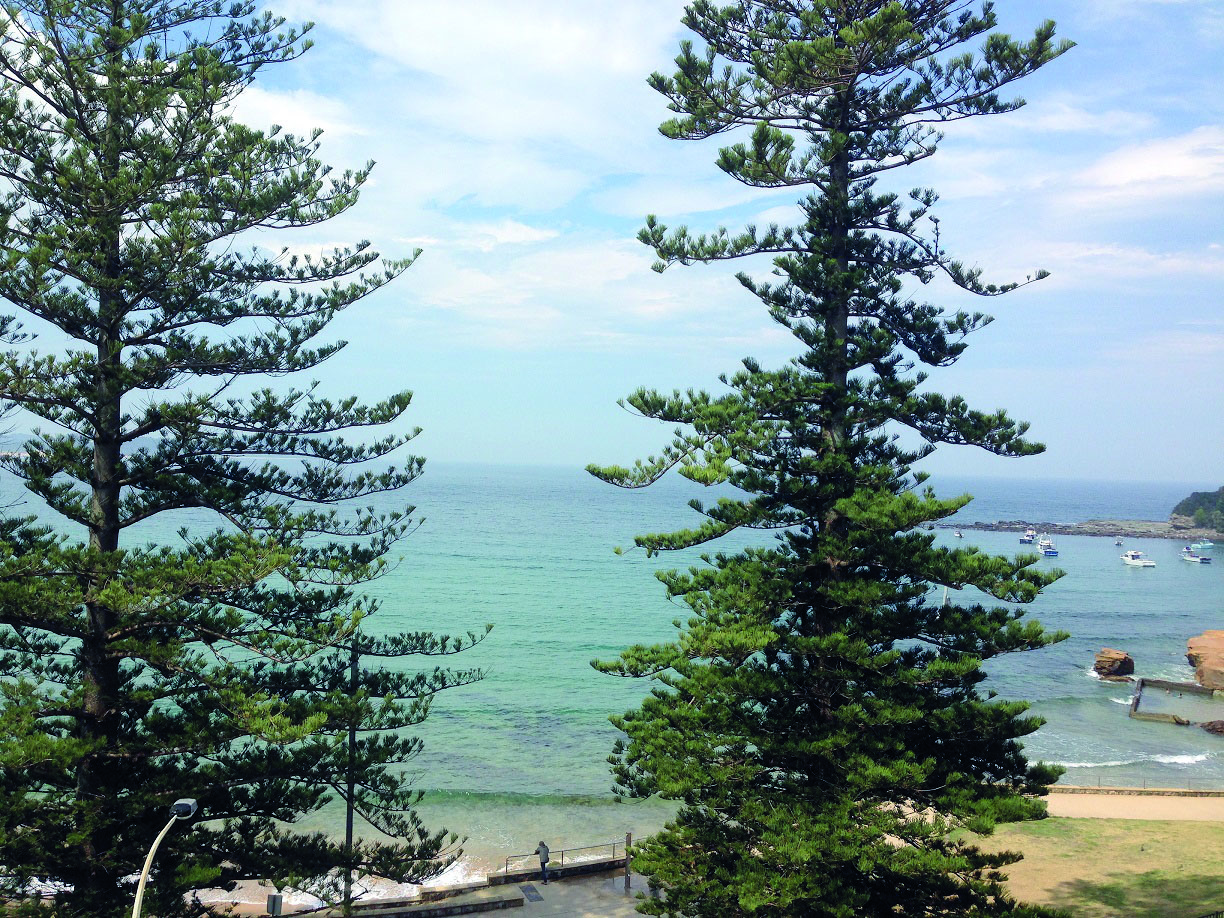
\includegraphics[width=\linewidth]{32-Hawkins-01}
	\caption{View from the AAA2016 conference location, overlooking Terrigal beach.
		{\normalfont\scriptsize \\ Photo by Jacqueline Matthews 2016
	}}
	\label{fig:32-Hawkins-01}
\end{figure}
View from the AAA2016 conference location, overlooking Terrigal beach. Photo by Jacqueline Matthews 2016.


\IJSRAsection{Prizes and AGM}
Each year at AAA conferences many prizes are handed out to celebrate and highlight people who have made outstanding contributions to archaeology in Australia. Three specific prizes focus on students; best student paper on archaeological science, best student paper on social archaeology and cultural heritage management, and the best student poster. These prizes seek to highlight the high quality of work undertaken by student researchers and also provide the winners with monetary prizes. The winning presentations ranged from geoarchaeology in Mongolia, to collaborative Aboriginal archaeology and high-school student perspectives of archaeology, showcasing the impressive diversity of research undertaken by Australian archaeology students. The 2016 student prize winners were:
 
\begin{description}
\item[Best Student Paper in Archaeological Science:]
	Anthea Vella (Flinders University) with Ian Moffat (Flinders University),
	Julia Clark (National Museum of Mongolia),
	David Putnam (University of Maine at Pesque Isle),
	Bayandelger Chinbold, (National Museum of Mongolia),
	Stefani Crabtree (Washington State University and Université de Franche-Comté) and Camilla Sturm (University of Pittsburgh)
	\enquote{Digital Geoarchaeological Investigations at the Soyo Archaeological Site, Northern Mongolia}
	
\item[Best Student Paper in Social Archaeology/Cultural Heritage Management:]
Joanne Thredgold (Flinders University) with Angus Giles,
Kane Johnson and George Tripp (all River Murray and Mallee Aboriginal Corporation) \enquote{Stone Artefacts and Earth Oven Mounds at Calperum Station,
the Riverland, South Australia}

\item[Best Student Poster:]
Brittany George (University of Western Australia)
\enquote{Western Australian high school students’ perceptions of archaeology}
\end{description}

The AAA Annual General Meeting (AGM) was held during the conference to discuss matters regarding the Association. Within the AAA there are two Student Representatives (one from the East coast and one from the West) who aim to support student members of the Association as well as the wider body of archaeology students across Australia. At the 2016 AGM, the Student Representatives discussed the successful running of the Student Research Grant Scheme in 2016, which is run annually by AAA and provides funding for student led research, and the importance of the National Archaeology Student Conference (NASC), which is not directly affiliated with AAA but aims to create a supportive platform for all archaeology students in Australia to present their research.

 \begin{figure}[!htb]
 	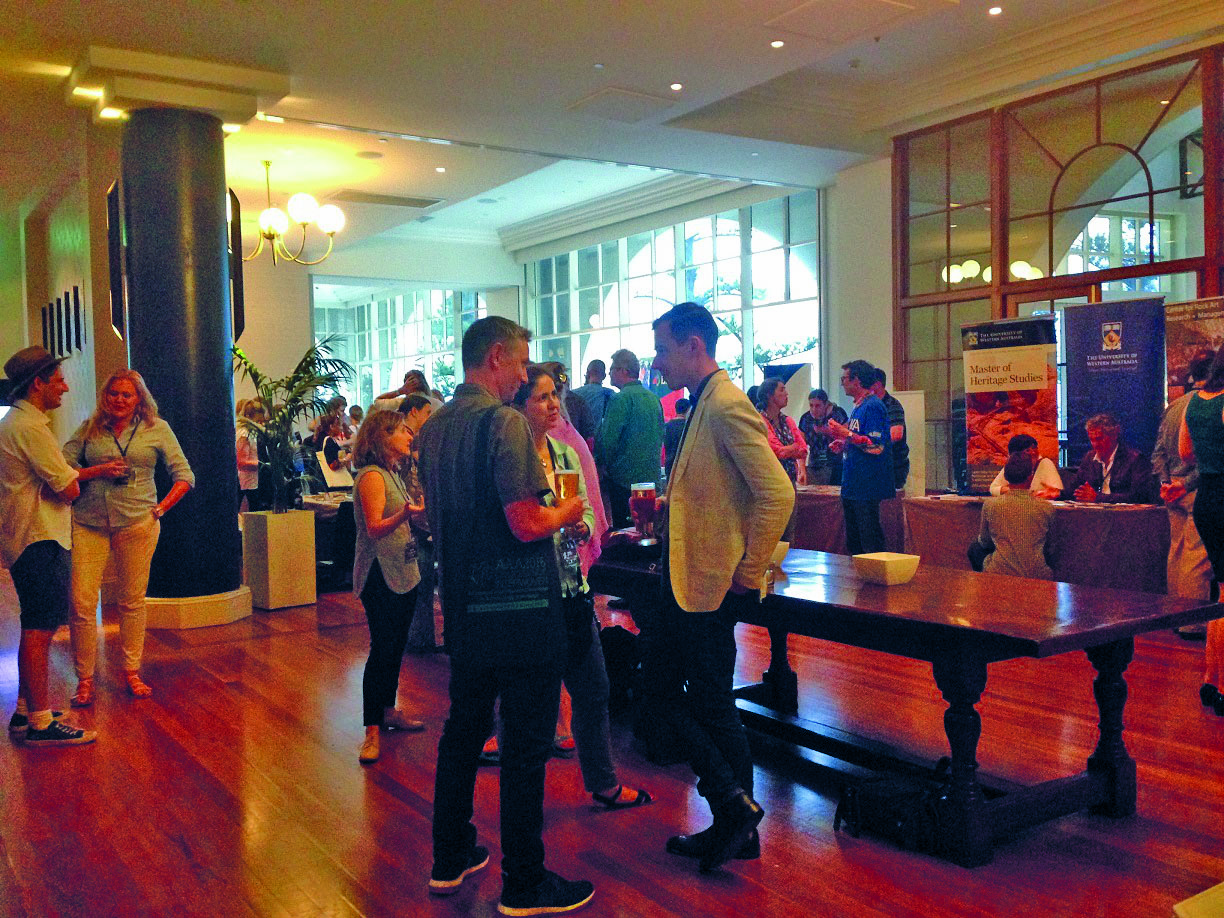
\includegraphics[width=\linewidth]{32-Hawkins-02}
 	\caption{The Meet the Graduates event was well attended by university departments, the private sector and students at AAA2016.
 		{\normalfont\scriptsize \\ Photo by Jacqueline Matthews 2016
 	}}
 	\label{fig:32-Hawkins-02}
 \end{figure}
 
\IJSRAsection{Student input}
Students are encouraged to be directly involved with the conference and, as mentioned above, the AAA provides travel grants for students who are presenting to help facilitate their attendance. Furthermore, volunteer opportunities are available at AAA conferences and for those who volunteer at the conference their registration fee is waived. At the 2016 conference, there were 7 volunteers; 4 students from the University of Sydney and 3 from the Darkinjung LALC. There were reasonable numbers of student presenters at the conference; out of the 110 paper presenters 33 were identified as students, 8 of the 20 posters were presented by students, and 6 of the 16 sessions were co-convened by postgraduate students.
 
The focus of the conference theme on collaboration between archaeologists and Indigenous communities highlights a crucial aspect of current and future Australian archaeology. However, such a focus does potentially have unintended consequences for potential student presenters, as many students as junior researchers (and particularly undergraduates) do not have the relevant experiences or relationships to contribute to such a theme. Given that funding constraints make it difficult to attend a conference without presenting, it is possible that students who had nothing to present that was linked to the conference theme did not attend and missed out on the valuable insights a theme of collaboration holds for all areas of archaeology. We would hope that this imbalance will be addressed at future conferences to ensure that the value of engaging with Indigenous archaeology and heritage, and collaboration with communities is encouraged amongst the entire archaeological community in Australia and particularly the next generations represented by students.



\IJSRAsection{Conclusion}
Overall, we felt that the AAA2016 conference was the most collaborative and inclusive AAA conference to date. Between the hosts, the theme, the keynote address and the overall content of the sessions, deeper collaboration and understanding across different knowledge systems was at the forefront of discussions. In future, we hope that conference themes will facilitate similarly high numbers of Indigenous delegates and enthusiasm for collaboration throughout archaeology, enabling closer and more mutually beneficial relationships between archaeologists and the communities with which they work. The level of student input and participation was good for a smaller national conference and we hope to see a continued increase, facilitated by the work of the AAA Student Representatives. We hope that other conferences around the world take note of the AAA2016 conference and follow their example to ensure more genuine collaboration with Indigenous communities.

\booltrue{nobib}%in case there are no references cited
\IJSRAclosing